\documentclass[11pt,a4paper]{article}

\usepackage{fontspec}
\setmainfont{Liberation Serif}
\setsansfont{Liberation Sans}

\usepackage{polyglossia}
\setmainlanguage{spanish}

\emergencystretch=3em

\usepackage[a4paper,margin=2.5cm]{geometry}
\usepackage{booktabs}
\usepackage{array}
\usepackage{xcolor}
\usepackage{enumitem}
\usepackage{caption}
\usepackage{graphicx}
\usepackage{hyperref}
\usepackage{xurl}
\usepackage{tabularx}
\usepackage{fancyhdr}

\hypersetup{
  colorlinks=true,
  linkcolor=blue!50!black,
  urlcolor=blue!50!black,
  citecolor=blue!50!black,
  pdftitle={Contaminación del aire en Lima Metropolitana -- Reporte},
  pdfauthor={Cartagena Valera Brush, Davis Leonardo; Lavado Torres, Gianmarco Gabriel; Chilon Tintaya, Monica Isabel; Huayta Esteban, Piero Alessandro}
}

\pagestyle{fancy}
\fancyhf{}
\fancyhead[L]{\small Dos Limas, un mismo cielo}
\fancyhead[R]{\small Minería de Datos -- UNMSM-FISI, 2026-I}
\fancyfoot[C]{\thepage}
\renewcommand{\headrulewidth}{0.4pt}

\title{\textbf{Contaminación del aire en Lima Metropolitana}\\[0.3em]
\large ``Dos Limas, un mismo cielo'': clustering y predicción de calidad del aire}
\author{
Cartagena Valera Brush, Davis Leonardo \and
Lavado Torres, Gianmarco Gabriel \and
Chilon Tintaya, Monica Isabel \and
Huayta Esteban, Piero Alessandro
}
\date{Minería de Datos -- UNMSM-FISI, 2026-I}

\begin{document}
\renewcommand{\tablename}{Tabla}

\maketitle
\thispagestyle{fancy}

\vspace{-1.5em}
\begin{center}
\small Fuente de datos: SENAMHI -- \emph{Monitoreo de los contaminantes del aire en Lima Metropolitana}\footnote{\url{https://www.datosabiertos.gob.pe/dataset/datos-horarios-de-contanimantes-del-aire-en-lima-metropolitana-servicio-nacional-de}}
(Plataforma Nacional de Datos Abiertos del Perú). Dataset horario, 10 estaciones, ventana analizada
2014-10-01 a 2020-09-30 (514{,}680 registros hora-estación).
\end{center}

\vspace{1em}

% =====================================================================
\section{Contexto y problema}
% =====================================================================

Lima Metropolitana no respira el mismo aire en todas sus zonas. Los datos horarios de
material particulado fino (PM2.5) publicados por SENAMHI para 10 estaciones de
monitoreo muestran una brecha sostenida entre distritos: estaciones del este y norte de
la ciudad --ATE (39.4~\textmu g/m\textsuperscript{3}), Puente Piedra (31.2), San Juan de
Lurigancho (29.9), Santa Anita (29.1) y Huachipa (28.3)-- registran un promedio
histórico de PM2.5 por encima del Estándar de Calidad Ambiental (ECA) anual de
25~\textmu g/m\textsuperscript{3} fijado por el D.S.\ N.\textdegree~003-2017-MINAM,
mientras que las 5 estaciones restantes (Villa María del Triunfo, Carabayllo, Campo de
Marte, San Martín de Porres, San Borja) quedan por debajo; ninguna estación supera, en
promedio, el ECA de 24h (50~\textmu g/m\textsuperscript{3}). Esta desigualdad espacial
es la tesis que atraviesa el proyecto: \emph{dos Limas, un mismo cielo}.

El problema es relevante para el contexto peruano en dos frentes. Primero, de
\textbf{salud pública}: la exposición crónica a PM2.5 está asociada por la evidencia
científica internacional a enfermedades respiratorias y cardiovasculares, y las zonas
más expuestas de Lima no cuentan hoy con un sistema accesible que traduzca los datos
crudos de SENAMHI en una alerta interpretable. Segundo, de \textbf{gestión ambiental}:
sin una segmentación clara de qué estaciones concentran el problema ni un pronóstico de
su evolución estacional (el llamado ``invierno limeño''), es difícil priorizar dónde
enfocar campañas de mitigación o monitoreo adicional con recursos limitados.

\textbf{A quién beneficia:} autoridades ambientales y de salud (MINAM, SENAMHI, gobiernos
locales de los distritos más expuestos) que necesitan priorizar intervención con datos, y
la ciudadanía de las zonas identificadas como de mayor riesgo, que hoy no tiene acceso a
una herramienta simple para consultar el estado de la calidad del aire de su zona.

\textbf{Costo de no resolverlo:} sin segmentación ni pronóstico, la asignación de
recursos de monitoreo y mitigación se hace a ciegas, tratando a Lima como una sola zona
homogénea cuando la evidencia (Sección~4 y~5) muestra que no lo es. Un sistema que
clasifique horas de riesgo y proyecte la tendencia mensual permite, como mínimo,
anticipar picos estacionales con semanas de margen en vez de reaccionar después del
hecho.

% =====================================================================
\section{Objetivos SMART}
% =====================================================================

Los siguientes objetivos están anclados a resultados ya obtenidos y verificables en el
proyecto (\texttt{models/\allowbreak metrics.json}, \texttt{models/\allowbreak forecast\_metrics.json} y el
código fuente citado), no son metas genéricas de relleno.

\begin{enumerate}[label=\textbf{O\arabic*.}, leftmargin=2.2em]

\item \textbf{Clasificación de horas de alta contaminación.} Entrenar y desplegar,
para la presentación de la semana~16 (S16) del curso, un clasificador binario de horas
con PM2.5 por encima del ECA de 24h (50~\textmu g/m\textsuperscript{3}) que alcance un
F1 $\geq 0.40$ en la clase minoritaria sobre un hold-out cronológico agrupado por día
calendario, auditable en \texttt{models/\allowbreak metrics.json}.
\emph{Estado: ya cumplido} -- el modelo desplegado (\texttt{rf\_classweight}) obtiene
F1 = 0.419 (Sección~4).

\item \textbf{Pronóstico mensual de PM2.5.} Producir, para S16, un pronóstico de al
menos 4 períodos futuros de PM2.5 mensual con un error porcentual medio (MAPE)
$\leq 10\%$ sobre un hold-out de 12 meses sin barajar, auditable en
\texttt{models/\allowbreak forecast\_metrics.json}.
\emph{Estado: ya cumplido} -- el modelo ganador (naive estacional) obtiene
MAPE = 8.18\% en un pronóstico de 6 meses (Sección~4).

\item \textbf{Segmentación espacial de estaciones.} Agrupar, para S16, las 10
estaciones SENAMHI en al menos 2 clusters con coeficiente de silueta positivo, para
sustentar cuantitativamente la desigualdad de ``las dos Limas'' entre zonas.
\emph{Estado: ya cumplido} -- K-means con $k=2$ sobre el perfil estandarizado de
contaminantes por estación obtiene silueta = 0.330 (inercia = 30.1).

\item \textbf{Trazabilidad de consultas.} Implementar, para S16, un CRUD accesible
desde el navegador sin credenciales que registre cada consulta de predicción (entrada +
resultado del Objetivo~O1) con timestamp automático, permitiendo editar y eliminar
registros.
\emph{Estado: ya cumplido} -- CRUD funcional sobre SQLite (\texttt{data/\allowbreak consultas.db})
con las 4 operaciones, integrado como Panel~4 de \texttt{app.py}.

\end{enumerate}

% =====================================================================
\section{KPIs del proyecto}
% =====================================================================

Todos los valores de \emph{baseline} de esta tabla provienen directamente de los
artefactos versionados del proyecto (\texttt{models/\allowbreak metrics.json} y
\texttt{models/\allowbreak forecast\_metrics.json}, generados el 2026-07-21) o de un cálculo en
vivo sobre \texttt{data/\allowbreak air\_contamination\_clean.parquet}; ninguno es inventado. Las
\emph{metas} son objetivos de mejora incremental sobre ese baseline, propuestos como
referencia para las próximas iteraciones del proyecto.

\begin{table}[h!]
\centering
\small
\begin{tabular}{@{}>{\raggedright\arraybackslash}p{0.50\textwidth}
                  >{\centering\arraybackslash}p{0.16\textwidth}
                  >{\centering\arraybackslash}p{0.16\textwidth}@{}}
\toprule
\textbf{KPI} & \textbf{Baseline (real)} & \textbf{Meta} \\
\midrule
F1 de la clase ``alta contaminación'' (modelo desplegado, \texttt{rf\_classweight}) &
0.419 & $\geq 0.45$ \\[0.6em]
Recall de la clase ``alta contaminación'' (mismo modelo) &
77.8\% & $\geq 85\%$ \\[0.6em]
MAPE del pronóstico mensual de PM2.5 (modelo ganador, naive estacional, hold-out 12 meses) &
8.18\% & $\leq 7\%$ \\[0.6em]
Cobertura de dato medido (no imputado) de PM2.5, a nivel de todo el dataset limpio &
62.2\% / 37.8\% imp. & imp.\ $\leq 30\%$ \\
\bottomrule
\end{tabular}
\caption{KPIs propuestos con baseline real verificado y metas de mejora incremental
para las próximas iteraciones del proyecto.}
\end{table}

El cuarto KPI (cobertura de dato medido) es distinto de los otros tres: no depende de
un modelo, sino de la infraestructura de monitoreo de SENAMHI -- mejorarlo requeriría
menos huecos de sensor en campo, no un cambio de algoritmo. Se incluye porque delimita
qué tan confiables son los otros KPIs: un F1 o un MAPE calculados sobre una serie con
37.8\% de datos imputados heredan parte de esa incertidumbre.

% =====================================================================
\section{Justificación de modelos}
% =====================================================================

\subsection{Segmentación de estaciones: selección de $k$}
\label{sec:clustering-just}

La unidad de clustering es la \emph{estación}, no la hora: cada uno de los 10 puntos
que entra a K-means es el promedio histórico de sus 6 contaminantes (PM10, PM2.5,
SO\textsubscript{2}, NO\textsubscript{2}, O\textsubscript{3}, CO) a lo largo de toda
la ventana analizada. Los 6 promedios se estandarizan con \texttt{StandardScaler}
antes de agrupar, para que ningún contaminante domine el agrupamiento solo por su
escala (CO, en \textmu g/m\textsuperscript{3}, tiene un orden de magnitud mucho mayor
que el resto). Se usa \texttt{SEED = 96} (la misma semilla que el resto del proyecto)
para que el resultado sea reproducible.

Se eligió $k=2$: con ese valor la silueta es 0.330 (positiva, clusters razonablemente
separados), frente a 0.297 con $k=3$ -- sumar un tercer grupo no mejora la separación,
solo fragmenta las 10 estaciones en particiones más pequeñas y ruidosas. Esta silueta
se calcula sobre solo 10 puntos (una fila por estación): con tan pocos puntos, subir
$k$ tiende a dejar grupos de 1--2 miembros, lo que la vuelve más ruidosa, y por eso
\textbf{no es directamente comparable} con la silueta calculada a nivel de fila-hora
en el notebook de EDA (\textasciitilde 515{,}000 registros) -- aunque en la práctica
ambas coinciden en que $k=2$ es el mejor valor.

\begin{table}[h!]
\centering
\small
\begin{tabular}{@{}lcccccc@{}}
\toprule
\textbf{Cluster} & \textbf{pm\_10} & \textbf{pm\_25} & \textbf{so2} & \textbf{no2} & \textbf{o3} & \textbf{co} \\
\midrule
0 (baja contaminación) & 65.0 & 19.3 & 7.0 & 19.3 & 16.6 & 678.6 \\
1 (alta contaminación) & 92.7 & 31.6 & 14.9 & 30.7 & 12.3 & 1026.6 \\
\bottomrule
\end{tabular}
\caption{Perfil promedio de contaminantes por cluster ($k=2$), unidades originales de cada contaminante.}
\label{tab:cluster-profile}
\end{table}

\textbf{Conclusión razonada.} El cluster de alta contaminación es entre un 40\% y
más del doble más alto que el de baja en todos los contaminantes, con una excepción:
el O\textsubscript{3}, más bajo (12.3 vs.\ 16.6) -- consistente con que el ozono es un
contaminante secundario y fotoquímico (se forma en la atmósfera bajo luz solar y tiende
a consumirse por titulación con los óxidos de nitrógeno del tráfico), no uno que se
emita directamente como los demás. Las 5 estaciones del cluster de alta contaminación
(ATE, Huachipa, Puente Piedra, San Juan de Lurigancho, Santa Anita) coinciden
\emph{exactamente} con las 5 estaciones que superan el ECA anual de 25~\textmu
g/m\textsuperscript{3} en la Sección~1 -- dos métodos completamente distintos
(clustering no supervisado vs.\ un umbral regulatorio fijo) llegando al mismo
resultado.

\subsection{Clasificación: RF (class\_weight) vs. XGBoost vs. RF+SMOTE}
\label{sec:clasificacion}

La variable objetivo (\texttt{PM2.5 > 50~\textmu g/m\textsuperscript{3}}, ECA de 24h)
está fuertemente desbalanceada: solo el 7.9\% de las horas medidas son ``alta
contaminación''. Las features son los 5 contaminantes restantes
(\texttt{pm\_10, so2, no2, o3, co}), \texttt{hora}, \texttt{mes}, \texttt{estacion}
(codificada con one-hot dentro del propio \texttt{Pipeline} del modelo,
\texttt{src/\allowbreak models.py}, función \texttt{\_preprocesador}) y la media móvil
de las 3h \textbf{anteriores} de cada contaminante por estación (rezago -- captura la
acumulación previa a un pico, no solo el instante puntual; función
\texttt{\_agregar\_rezago}, líneas 39--46). Se entrenaron y evaluaron tres estrategias
sobre el mismo hold-out (30\% de test, separado por día calendario para no filtrar
horas del mismo día entre train y test; función \texttt{dividir}, líneas 70--82,
aplicada en las líneas 261--262):

\begin{table}[h!]
\centering
\small
\resizebox{\textwidth}{!}{%
\begin{tabular}{@{}lccccc@{}}
\toprule
\textbf{Modelo} & \textbf{Accuracy} & \textbf{ROC-AUC} & \textbf{F1 (alta)} & \textbf{Recall (alta)} & \textbf{Precision (alta)} \\
\midrule
RF + class\_weight & 0.875 & 0.938 & 0.517 & 0.840 & 0.374 \\
\textbf{XGBoost + scale\_pos\_weight} (ganador) & 0.880 & \textbf{0.943} & 0.531 & 0.850 & 0.386 \\
RF + SMOTE (referencia, no desplegado) & \textbf{0.926} & 0.940 & \textbf{0.605} & 0.706 & \textbf{0.529} \\
\bottomrule
\end{tabular}%
}
\caption{Métricas sobre la clase minoritaria (``alta contaminación''), $n_{test}=93{,}793$ horas.}
\end{table}

\textbf{Conclusión razonada.} El modelo se elige por \textbf{F1 de la clase
minoritaria}, no por accuracy: en un problema con 92.1\% de horas ``baja'' un
clasificador trivial que siempre prediga ``baja'' ya obtendría accuracy alto sin ser
útil. El costo de no avisar una hora contaminada (falso negativo) es mayor que el de
una falsa alarma (falso positivo), por lo que el recall de la clase alta pesa más que
la precisión global. \texttt{RF + SMOTE} obtiene el F1 más alto de los tres (0.605 vs.\
0.531), pero el proyecto lo excluye deliberadamente de la comparación de ``mejor
modelo desplegable'' (\texttt{src/\allowbreak models.py}, función \texttt{entrenar\_y\_evaluar\_todo},
líneas 274--276, que descartan expresamente el candidato \texttt{rf\_smote} antes de
fijar el mejor modelo):
se entrena únicamente como referencia académica del efecto del sobremuestreo sobre el
recall, no se serializa como artefacto de despliegue, y su mejora de F1 sobre
\texttt{xgb\_scaleposw} (+0.074) no compensa la complejidad añadida de mantener en
producción un pipeline de SMOTE. El modelo ganador y efectivamente servido por el
Panel~2 es, por lo tanto, \textbf{\texttt{xgb\_scaleposw}}, coherente entre
\texttt{models.py}, \texttt{metrics.json} y \texttt{panel\_predictivo.py}.

La interpretabilidad se resuelve con SHAP (\texttt{TreeExplainer}): el
\emph{summary plot} (Figura~\ref{fig:shap-summary}) muestra qué contaminantes mueven
más la predicción a nivel global, y el \emph{force plot} (Figura~\ref{fig:shap-force})
descompone una predicción puntual. Ambos dan sentido físico a la decisión del modelo
-- relevante frente a la pregunta de causalidad vs.\ correlación que el curso exige
poder responder.

\begin{figure}[h!]
\centering
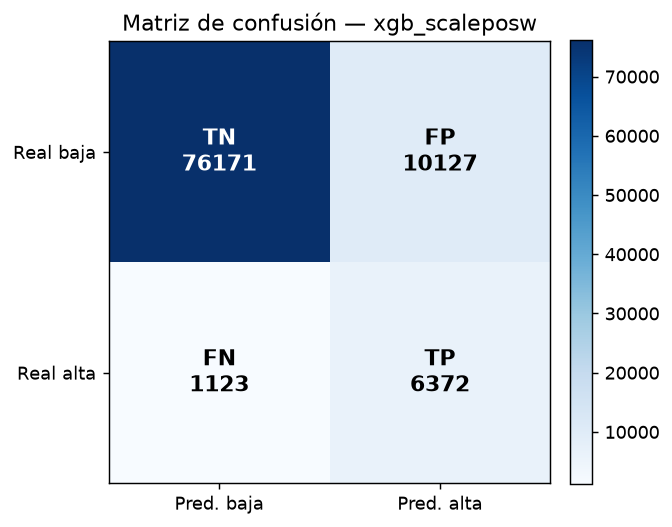
\includegraphics[width=0.75\textwidth]{../models/confusion_matrix.png}
\caption{Matriz de confusión del modelo ganador (\texttt{xgb\_scaleposw}).}
\label{fig:confmat}
\end{figure}

\begin{figure}[h!]
\centering
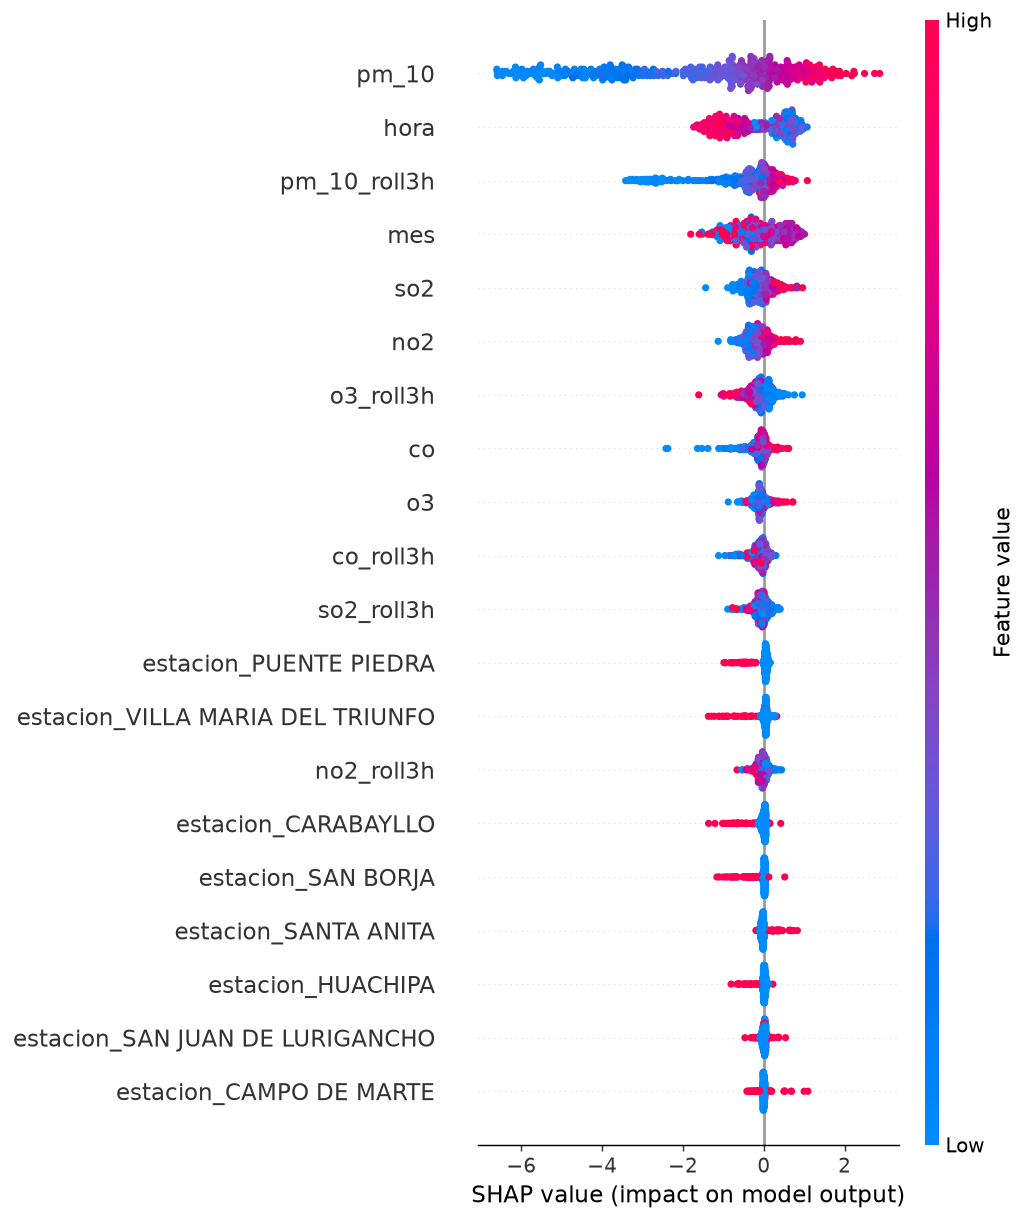
\includegraphics[width=0.75\textwidth]{../models/xgb_scaleposw_shap_summary.png}
\caption{SHAP summary plot (importancia global de features) del modelo ganador.}
\label{fig:shap-summary}
\end{figure}

\begin{figure}[h!]
\centering
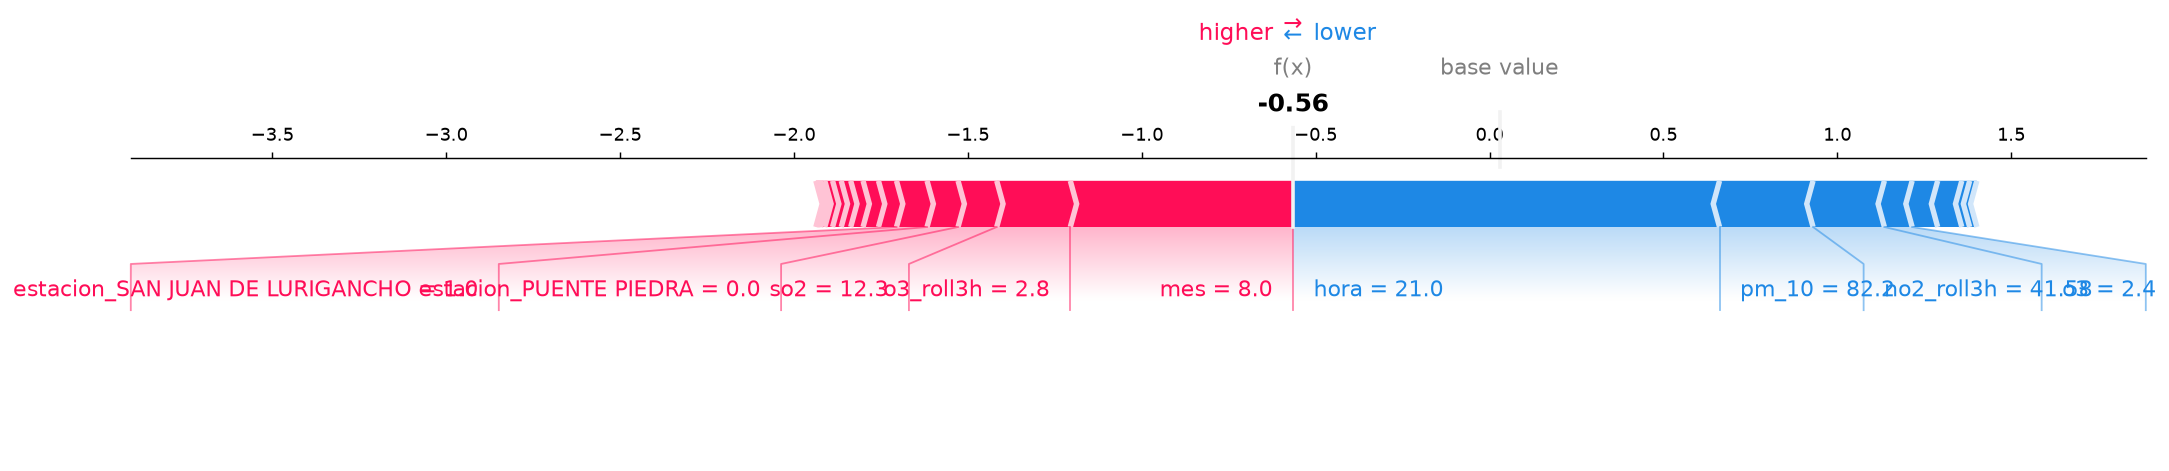
\includegraphics[width=0.85\textwidth]{../models/xgb_scaleposw_shap_force.png}
\caption{SHAP force plot para un caso puntual real: estación San Juan de Lurigancho, 2020-08-28 21:00.}
\label{fig:shap-force}
\end{figure}

El caso de la Figura~\ref{fig:shap-force} es una hora real del set de test (estación
San Juan de Lurigancho, 2020-08-28 21:00, PM2.5 \textbf{medido} = 33.0~\textmu
g/m\textsuperscript{3}, por debajo del ECA de 24h). Con entrada
\texttt{pm\_10=82.2}, \texttt{so2=12.3}, \texttt{no2=40.3}, \texttt{o3=2.4},
\texttt{co=717.6}, \texttt{hora=21}, \texttt{mes=8}, \texttt{estacion=SAN JUAN DE
LURIGANCHO} y rezagos de 3h (\texttt{no2\_roll3h=41.6}, \texttt{o3\_roll3h=2.8} entre
otros), el modelo predice una probabilidad de 0.362 para ``alta contaminación'' --
por debajo del umbral de 0.5, así que clasifica correctamente esta hora como
\emph{baja}, coincidiendo con la etiqueta real. El mayor empuje hacia ``baja''
(azul) viene de \texttt{hora=21} ($-1.23$), seguido de \texttt{pm\_10=82.2} ($-0.27$) y
del \texttt{no2\_roll3h=41.6} ($-0.21$): aunque el PM10 está elevado y es hora punta
nocturna, tanto el efecto SHAP puntual de la hora como el del PM10 empujan hacia la
clase baja, no hacia la alta -- evidencia de que el modelo no aplica un umbral
univariado simple sobre un solo contaminante, sino que pondera la combinación completa
de contaminantes, momento del día, estación y tendencia reciente. Lo que empuja hacia
``alta'' (rojo) es \texttt{mes=8} (invierno limeño, $+0.64$), el
\texttt{o3\_roll3h=2.8} muy bajo ($+0.21$) y el \texttt{so2=12.3} ($+0.11$), pero no
alcanza para revertir el resultado.

\subsection{Pronóstico: naive estacional vs. Holt-Winters vs. SARIMA}
\label{sec:pronostico}

Para el PM2.5 mensual se compararon tres modelos sobre un hold-out cronológico de 12
meses (sin barajar, para no filtrar futuro hacia el pasado):

\begin{table}[h!]
\centering
\small
\begin{tabular}{@{}lccc@{}}
\toprule
\textbf{Modelo} & \textbf{MAPE} & \textbf{RMSE} & \textbf{MAE} \\
\midrule
\textbf{Naive estacional} (ganador) & \textbf{8.18\%} & 2.34 & 2.04 \\
SARIMA & 11.30\% & 3.26 & 2.91 \\
Holt-Winters & 11.86\% & 3.30 & 3.03 \\
\bottomrule
\end{tabular}
\caption{Comparación de modelos de pronóstico, serie mensual agregada ``TODAS'' las estaciones, $n=67$ meses, hold-out=12.}
\end{table}

\textbf{Conclusión razonada.} El baseline más simple (repetir el valor del mismo mes
del ciclo anterior) supera a SARIMA y Holt-Winters en esta serie. Con solo 55 puntos de
entrenamiento y una estacionalidad mensual regular (el ``invierno limeño''), los
modelos con más parámetros no logran capturar patrón adicional que no esté ya explicado
por la estacionalidad pura, y terminan sobreajustando ruido de corto plazo. Esta es una
conclusión honesta del proyecto, no una limitación oculta: un modelo más sofisticado no
siempre es la mejor respuesta cuando la serie es corta y muy estacional.

El pronóstico final (6 meses, mayo--octubre) se reajusta con el modelo ganador sobre
toda la serie disponible --no solo sobre el tramo de entrenamiento del hold-out-- y
proyecta valores entre \textbf{25 y 31~\textmu g/m\textsuperscript{3}}. Como es un
promedio mensual, el umbral que corresponde para juzgarlo es el ECA \textbf{anual} de
largo plazo (25~\textmu g/m\textsuperscript{3}, Sección~1), no el de 24h
(50~\textmu g/m\textsuperscript{3}): contra ese umbral correcto, el pronóstico queda al
borde o ligeramente por encima, no cómodamente por debajo -- una señal de alerta
temprana concreta para la temporada de invierno limeño.

% =====================================================================
\section{Narrativa: de la complicación a la resolución}
% =====================================================================

\subsection*{(a) Situación}

El dataset crudo de SENAMHI cubre 10 estaciones de monitoreo de Lima Metropolitana con
registros horarios de 6 contaminantes (PM10, PM2.5, SO\textsubscript{2},
NO\textsubscript{2}, O\textsubscript{3}, CO). Tras la limpieza, la ventana analizada es
2014-10-01 a 2020-09-30, con 514{,}680 filas hora-estación.

\subsection*{(b) Complicación real en los datos}

\begin{enumerate}[leftmargin=1.5em]

\item \textbf{Vacío estructural anterior a octubre de 2014.} PM2.5 tiene entre 50\% y
58\% de nulos antes de esa fecha, y recién baja a 22.7\% de nulos en octubre de 2014.
No es un hueco puntual: es la propia serie histórica siendo demasiado incompleta para
imputar con confianza. Por eso el proyecto define \texttt{FECHA\_CORTE = 2014-10-01} y
descarta todo lo anterior en vez de rellenarlo (\texttt{src/\allowbreak preprocessing.py}, líneas
39--45).

\item \textbf{Apagón de sensor de más de un año en SAN MARTIN DE PORRES.} Esa estación
concentra dos huecos largos: de 2018-08-06 a 2019-05-16 (\textasciitilde 9.4 meses) y,
más grave, de 2019-07-10 hasta el final de la serie (2020-09-30), \textasciitilde 15
meses consecutivos sin dato medido. En total, 42.5\% de las horas de esa estación son
imputadas por climatología (contra 37.8\% de imputación a nivel global del dataset) --
sus últimos 15 meses de serie no son observación real, sino relleno estacional
estimado a partir de años previos.

\item \textbf{Fuga de autocorrelación temporal en la validación.} Un split
aleatorio fila-por-fila del dataset horario deja horas del mismo día calendario
repartidas entre train y test. Como los contaminantes de horas consecutivas del mismo
día están fuertemente correlacionados, esto infla de forma optimista el ROC-AUC/F1
reportado -- el modelo ``ve'' parcialmente el día que se le pide predecir.

\item \textbf{Desbalance de clases en la etiqueta de alta contaminación.} Solo 7.9\% de
las horas medidas superan el ECA de 24h; un modelo entrenado sin ajuste alguno tendería
a ignorar la clase minoritaria, que es precisamente la que importa para una alerta.

\end{enumerate}

\subsection*{(c) Resolución con técnicas del curso}

\begin{enumerate}[leftmargin=1.5em]

\item El vacío estructural (b.1) se resuelve por diseño: se recorta la ventana de
análisis en vez de imputar sobre una señal demasiado ruidosa para confiar en ella.

\item El apagón de SAN MARTIN DE PORRES (b.2) se resuelve con un pipeline de
imputación en 3 niveles, de más a menos confiable: interpolación lineal acotada a 6
horas para huecos cortos, climatología fina (mediana por estación-mes-hora) para
capturar estacionalidad, y climatología gruesa (mediana por estación-hora) como
respaldo final. Cada valor imputado queda marcado en una columna \texttt{\_imputado}
\emph{antes} de imputar, para que ningún panel del dashboard confunda dato real con
relleno (visible como métrica explícita en el Panel~1).

\item La fuga de autocorrelación (b.3) se resuelve reemplazando el split aleatorio por
un \texttt{Group\-Shuffle\-Split} agrupado por día calendario
(\texttt{src/\allowbreak models.py}, función \texttt{dividir}, líneas 132--156, aplicado en la
línea 536--537): todas las horas de un mismo día caen enteras en train o en test, nunca
repartidas.

\item El desbalance (b.4) se resuelve comparando explícitamente tres estrategias
(\texttt{class\_\allowbreak weight}, \texttt{scale\_\allowbreak pos\_\allowbreak weight}, SMOTE) y eligiendo por F1 de la
clase minoritaria en vez de accuracy (Sección~\ref{sec:clasificacion}), documentando
por qué SMOTE no se despliega pese a ganar por F1 crudo.

\end{enumerate}

\subsection*{(d) Impacto: qué decisión real habilita}

Con estas resoluciones, el proyecto entrega tres piezas accionables: (1) una
clasificación de riesgo por hora con F1 = 0.531 y explicación SHAP, útil como insumo de
un sistema de alerta temprana explicable, no solo una etiqueta binaria; (2) un
pronóstico mensual con 8.18\% de error que proyecta 25--31~\textmu
g/m\textsuperscript{3} para el próximo invierno limeño --al borde o por encima del ECA
anual--, suficiente para anticipar con semanas de antelación el pico estacional y
planificar campañas de salud pública o restricciones vehiculares estacionales; y (3)
una segmentación de estaciones
(silueta = 0.330 con $k=2$) que identifica objetivamente 5 zonas prioritarias (ATE,
Puente Piedra, San Juan de Lurigancho, Santa Anita, Huachipa) para concentrar inversión
en monitoreo y mitigación, en vez de tratar Lima como una sola zona homogénea.

\end{document}
